\documentclass[11pt, letterpaper]{article}

% Packages
\usepackage[margin=0.85in]{geometry}
\usepackage{booktabs, tabularx, float, multirow}
\usepackage{enumitem}
\usepackage{parskip}
\usepackage{tikz}
\usetikzlibrary{arrows.meta, positioning, fit, backgrounds, calc}
\usepackage{listings}
\usepackage{hyperref}
\usepackage{xcolor}

% Compact lists
\setlist{noitemsep, topsep=3pt, leftmargin=1.5em}

% Code listing style
\lstset{basicstyle=\ttfamily\footnotesize, breaklines=true, frame=single, xleftmargin=1em}

% Table row padding
\renewcommand{\arraystretch}{1.15}

\hypersetup{colorlinks=true, linkcolor=blue, urlcolor=blue}

% ── Title ─────────────────────────────────────────────────────
\title{%
    {\LARGE\bfseries ITCS5010 GenAI:ForgePilot}\\[0.3em]
    {\large CLI Coding Assistant --- Final Report}
}

\author{%
    \begin{tabular}[t]{ccc}
        Varad Paradkar & Nidhi Shah & Brinda Chinnaraji \\[0.3em]
        \multicolumn{3}{c}{Sai Kiran Jagini \quad Shar Adhiambo}
    \end{tabular}%
}

\date{\today}

\begin{document}
\maketitle

\tableofcontents
\newpage

\section{Introduction}

\textbf{ForgePilot} is a modular CLI coding assistant that combines an agentic loop,
provider abstraction, MCP tool orchestration, and a local RAG pipeline.
The system supports practical repository workflows such as file inspection, edits,
shell execution, and grounded responses using local vector retrieval.

This report presents the architecture, runtime diagrams, implementation details,
validation evidence, and limitations/future work.

Repository links:
\begin{itemize}
    \item \textbf{Project Repository:} \url{https://github.com/vradcar/GenAI-Group-Project-2}
    \item \textbf{Local report source:} \texttt{docs/FINAL\_REPORT.md}
\end{itemize}

\section{Design Goals and Scope}

\subsection{Primary Goals}
\begin{itemize}
    \item Provide an interactive CLI assistant for coding tasks (single-run and REPL).
    \item Support safe execution via explicit user confirmation mode and fast execution via auto mode.
    \item Integrate external and local tools through MCP with a consistent runtime interface.
    \item Ground responses with local document retrieval using a persistent vector store.
\end{itemize}

\subsection{Scope Boundaries}
\begin{itemize}
    \item In-scope: CLI workflows, local tooling, MCP integration, and local RAG retrieval.
    \item Out-of-scope: multi-tenant cloud architecture, custom model training, and full enterprise auth.
\end{itemize}

\section{System Architecture Overview}

The system follows a layered architecture with a user-facing CLI, a core agent/runtime
layer, and tool/data backends.

\begin{figure}[H]
\centering
\resizebox{0.98\textwidth}{!}{%
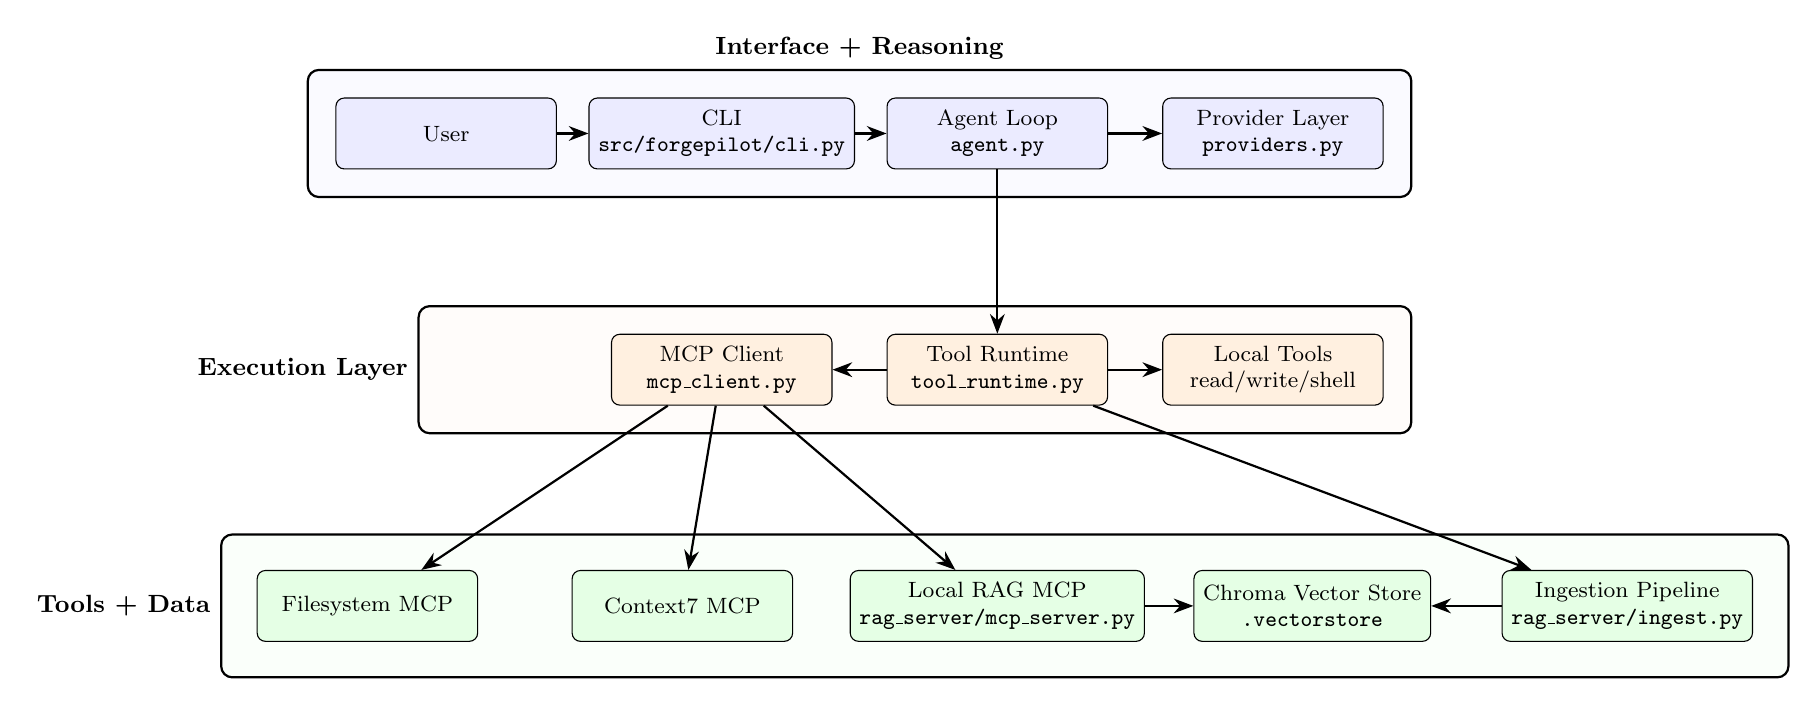
\begin{tikzpicture}[
    box/.style={rectangle, draw, rounded corners=3pt, minimum width=2.8cm,
                minimum height=0.9cm, align=center, font=\footnotesize},
    arr/.style={-{Stealth[length=2.5mm]}, thick}
]

% --- Grid Coordinates ---
% Top & Middle Row Columns (Gap = 3.5)
\def\cO{-5.0}  
\def\cI{-1.5}  
\def\cII{2.0}  
\def\cIII{5.5} 
\def\cIV{9.0}  

% Bottom Row Columns (Gap = 4.0 - manually spaced further apart)
\def\bO{-6.0}  % Shifted left
\def\bI{-2.0}  % Shifted left
\def\bII{2.0}  % Kept centered with the diagram
\def\bIII{6.0} % Shifted right
\def\bIV{10.0} % Shifted right

% Rows
\def\rO{0}     % Top row
\def\rI{-3.0}  % Middle row
\def\rII{-6.0} % Bottom row

% --- Top Row (Interface + Reasoning) ---
\node[box, fill=blue!8] (user)     at (\cO, \rO) {User};
\node[box, fill=blue!8] (cli)      at (\cI, \rO) {CLI\\\texttt{src/forgepilot/cli.py}};
\node[box, fill=blue!8] (agent)    at (\cII, \rO) {Agent Loop\\\texttt{agent.py}};
\node[box, fill=blue!8] (provider) at (\cIII, \rO) {Provider Layer\\\texttt{providers.py}};

% --- Middle Row (Execution Layer) ---
\node[box, fill=orange!12] (mcp)     at (\cI, \rI) {MCP Client\\\texttt{mcp\_client.py}};
\node[box, fill=orange!12] (runtime) at (\cII, \rI) {Tool Runtime\\\texttt{tool\_runtime.py}};
\node[box, fill=orange!12] (local)   at (\cIII, \rI) {Local Tools\\read/write/shell};

% --- Bottom Row (Tools + Data) - USING NEW \b COORDINATES ---
\node[box, fill=green!10] (fs)     at (\bO, \rII) {Filesystem MCP};
\node[box, fill=green!10] (cx)     at (\bI, \rII) {Context7 MCP};
\node[box, fill=green!10] (ragmcp) at (\bII, \rII) {Local RAG MCP\\\texttt{rag\_server/mcp\_server.py}};
\node[box, fill=green!10] (vdb)    at (\bIII, \rII) {Chroma Vector Store\\\texttt{.vectorstore}};
\node[box, fill=green!10] (ingest) at (\bIV, \rII) {Ingestion Pipeline\\\texttt{rag\_server/ingest.py}};

% --- Background Groups ---
\begin{scope}[on background layer]
    % Top Box
    \node[rectangle, draw, rounded corners=4pt, thick, fill=blue!2, inner sep=0.35cm,
          fit=(user)(provider), label={[font=\small\bfseries]above:Interface + Reasoning}] {};
          
    % Middle Box
    \node[rectangle, draw, rounded corners=4pt, thick, fill=orange!2, inner sep=0.35cm,
          fit=(mcp)(local)(user |- mcp), label={[font=\small\bfseries]left:Execution Layer}] {};
          
    % Bottom Box
    \node[rectangle, draw, rounded corners=4pt, thick, fill=green!2, inner sep=0.45cm,
          fit=(fs)(ingest), label={[font=\small\bfseries]left:Tools + Data}] {};
\end{scope}

% --- Arrows ---
% Top flow
\draw[arr] (user) -- (cli);
\draw[arr] (cli) -- (agent);
\draw[arr] (agent) -- (provider);

% Agent to Runtime 
\draw[arr] (agent) -- (runtime); 

% Runtime distribution
\draw[arr] (runtime) -- (mcp);   
\draw[arr] (runtime) -- (local); 
\draw[arr] (runtime) -- (ingest); 

% MCP distribution
\draw[arr] (mcp) -- (fs);     
\draw[arr] (mcp) -- (cx);     
\draw[arr] (mcp) -- (ragmcp); 

% RAG and Ingestion flow
\draw[arr] (ragmcp) -- (vdb); 
\draw[arr] (ingest) -- (vdb); 

\end{tikzpicture}%
}
\caption{ForgePilot runtime architecture using CLI, agent loop, provider abstraction, MCP, and local RAG.}
\end{figure}

\subsection{Component Responsibilities}

\begin{table}[H]
\centering\small
\begin{tabularx}{\textwidth}{@{}l X@{}}
\toprule
\textbf{Component} & \textbf{Responsibility} \\
\midrule
CLI (\texttt{cli.py}) & Accept user tasks, run single-task mode or REPL mode, display tool call status and outputs. \\
Agent Loop (\texttt{agent.py}) & Generate one-step plans, parse structured responses, dispatch actions, and iterate to completion. \\
Provider Layer (\texttt{providers.py}) & Create model-client abstraction across providers and apply fallback behavior when provider setup fails. \\
Tool Runtime (\texttt{tool\_runtime.py}) & Enforce \texttt{confirm}/\texttt{auto} mode and route calls to local tools or MCP tools. \\
MCP Client (\texttt{mcp\_client.py}) & Connect to MCP servers, discover tools, namespace tool names, and normalize responses. \\
RAG Modules (\texttt{rag\_server/*}) & Ingest docs, create embeddings, retrieve top-k grounded chunks, and expose retrieval via MCP tools. \\
\bottomrule
\end{tabularx}
\caption{High-level component responsibility map.}
\end{table}

\section{State Diagram}

\begin{figure}[H]
\centering
\resizebox{0.96\textwidth}{!}{%
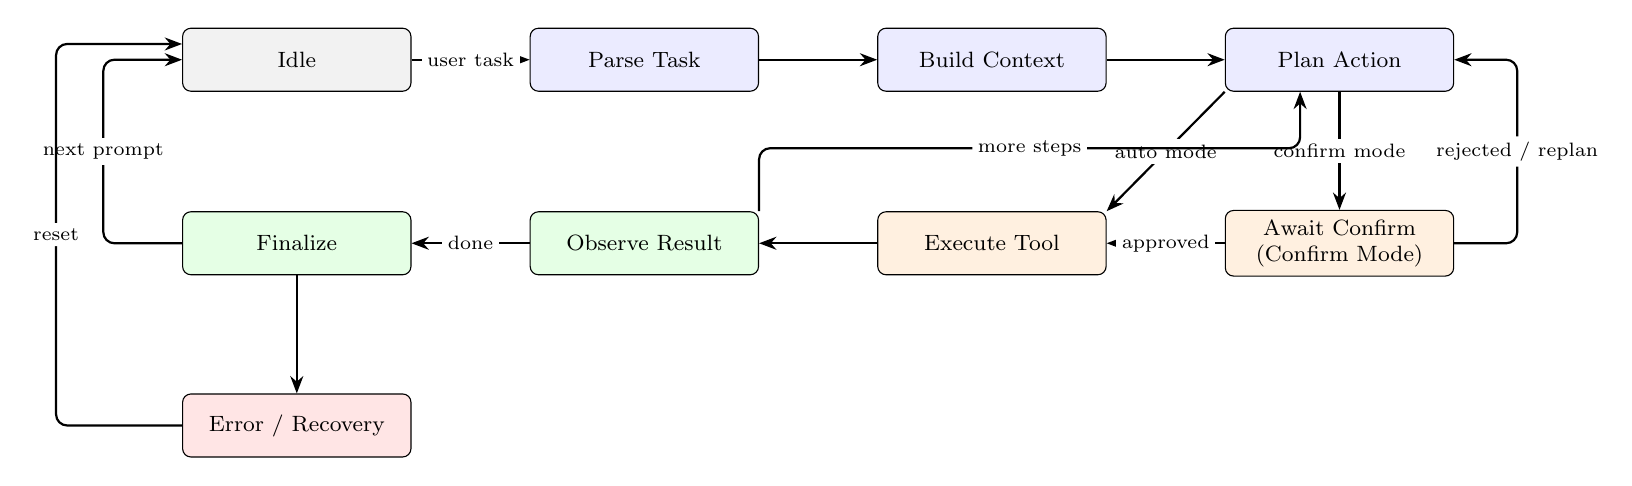
\begin{tikzpicture}[
  state/.style={rectangle, draw, rounded corners=3pt, minimum width=2.9cm, minimum height=0.8cm, align=center, font=\footnotesize},
  arr/.style={-{Stealth[length=2.2mm]}, thick},
  edgelabel/.style={fill=white, inner sep=2pt, font=\scriptsize},
  node distance=1.5cm and 1.5cm
]

% Top Row Nodes
\node[state, fill=gray!10] (idle) {Idle};
\node[state, fill=blue!8, right=of idle] (parse) {Parse Task};
\node[state, fill=blue!8, right=of parse] (ctx) {Build Context};
\node[state, fill=blue!8, right=of ctx] (plan) {Plan Action};

% Bottom Row Nodes (Aligned exactly under Top Row)
\node[state, fill=orange!12, below=of plan] (confirm) {Await Confirm\\(Confirm Mode)};
\node[state, fill=orange!12, left=of confirm] (exec) {Execute Tool};
\node[state, fill=green!10, left=of exec] (observe) {Observe Result};
\node[state, fill=green!10, left=of observe] (final) {Finalize};

% Error Node
\node[state, fill=red!10, below=of final] (error) {Error / Recovery};

% Standard Forward Flow Arrows
\draw[arr] (idle) -- node[edgelabel]{user task} (parse);
\draw[arr] (parse) -- (ctx);
\draw[arr] (ctx) -- (plan);
\draw[arr] (plan) -- node[edgelabel]{confirm mode} (confirm);
\draw[arr] (confirm) -- node[edgelabel]{approved} (exec);
\draw[arr] (exec) -- (observe);
\draw[arr] (observe) -- node[edgelabel]{done} (final);

% Auto Mode Diagonal (Plan to Exec)
\draw[arr] (plan.south west) -- node[edgelabel]{auto mode} (exec.north east);

% Feedback Loops & Routing 

% Rejected / Replan: Loops clearly out the right side
\draw[arr, rounded corners] (confirm.east) -- ++(0.8,0) |- node[edgelabel, near start]{rejected / replan} (plan.east);

% More Steps: Routes cleanly horizontally between the two rows
\draw[arr, rounded corners] (observe.north east) -- ++(0, 0.8) -| node[edgelabel, pos=0.25]{more steps} ([xshift=-0.5cm]plan.south);

% Return to Idle: Loops around the left side
\draw[arr, rounded corners] (final.west) -- ++(-1.0,0) |- node[edgelabel, near start]{next prompt} (idle.west);

% Error Flow
\draw[arr] (final.south) -- (error.north);

% Error Recovery: Loops wider around the left side to avoid the 'final' loop
\draw[arr, rounded corners] (error.west) -- ++(-1.6,0) |- node[edgelabel, near start]{reset} ([yshift=0.2cm]idle.west);

\end{tikzpicture}%
}
\caption{Agent execution lifecycle with confirm/auto branches and recovery path.}
\end{figure}

\section{Retrieval and MCP Pipeline}

\subsection{RAG Pipeline Summary}

\begin{itemize}
    \item Source docs from \texttt{docs/source\_docs} are chunked and embedded by \texttt{rag\_server/ingest.py}.
    \item Embeddings are persisted in Chroma under \texttt{.vectorstore}.
    \item \texttt{rag\_server/retriever.py} expands queries and performs fusion-style ranking.
    \item \texttt{rag\_server/mcp\_server.py} exposes \texttt{rag\_query\_docs} and \texttt{rag\_health}.
\end{itemize}

\subsection{MCP Server Roles}

\begin{table}[H]
\centering\small
\begin{tabularx}{\textwidth}{@{}l l X@{}}
\toprule
\textbf{Server} & \textbf{Type} & \textbf{Purpose} \\
\midrule
filesystem & MCP (Node) & File and directory operations in workspace scope. \\
context7 & MCP (remote) & External documentation/context retrieval for coding tasks. \\
rag & MCP (local Python) & Grounded retrieval from local vector store and health checks. \\
\bottomrule
\end{tabularx}
\caption{Configured MCP servers and their roles.}
\end{table}

\section{Sequence Diagram --- Scenario 1 (Documentation Query with RAG)}

\begin{figure}[H]
\centering
\resizebox{\textwidth}{!}{%
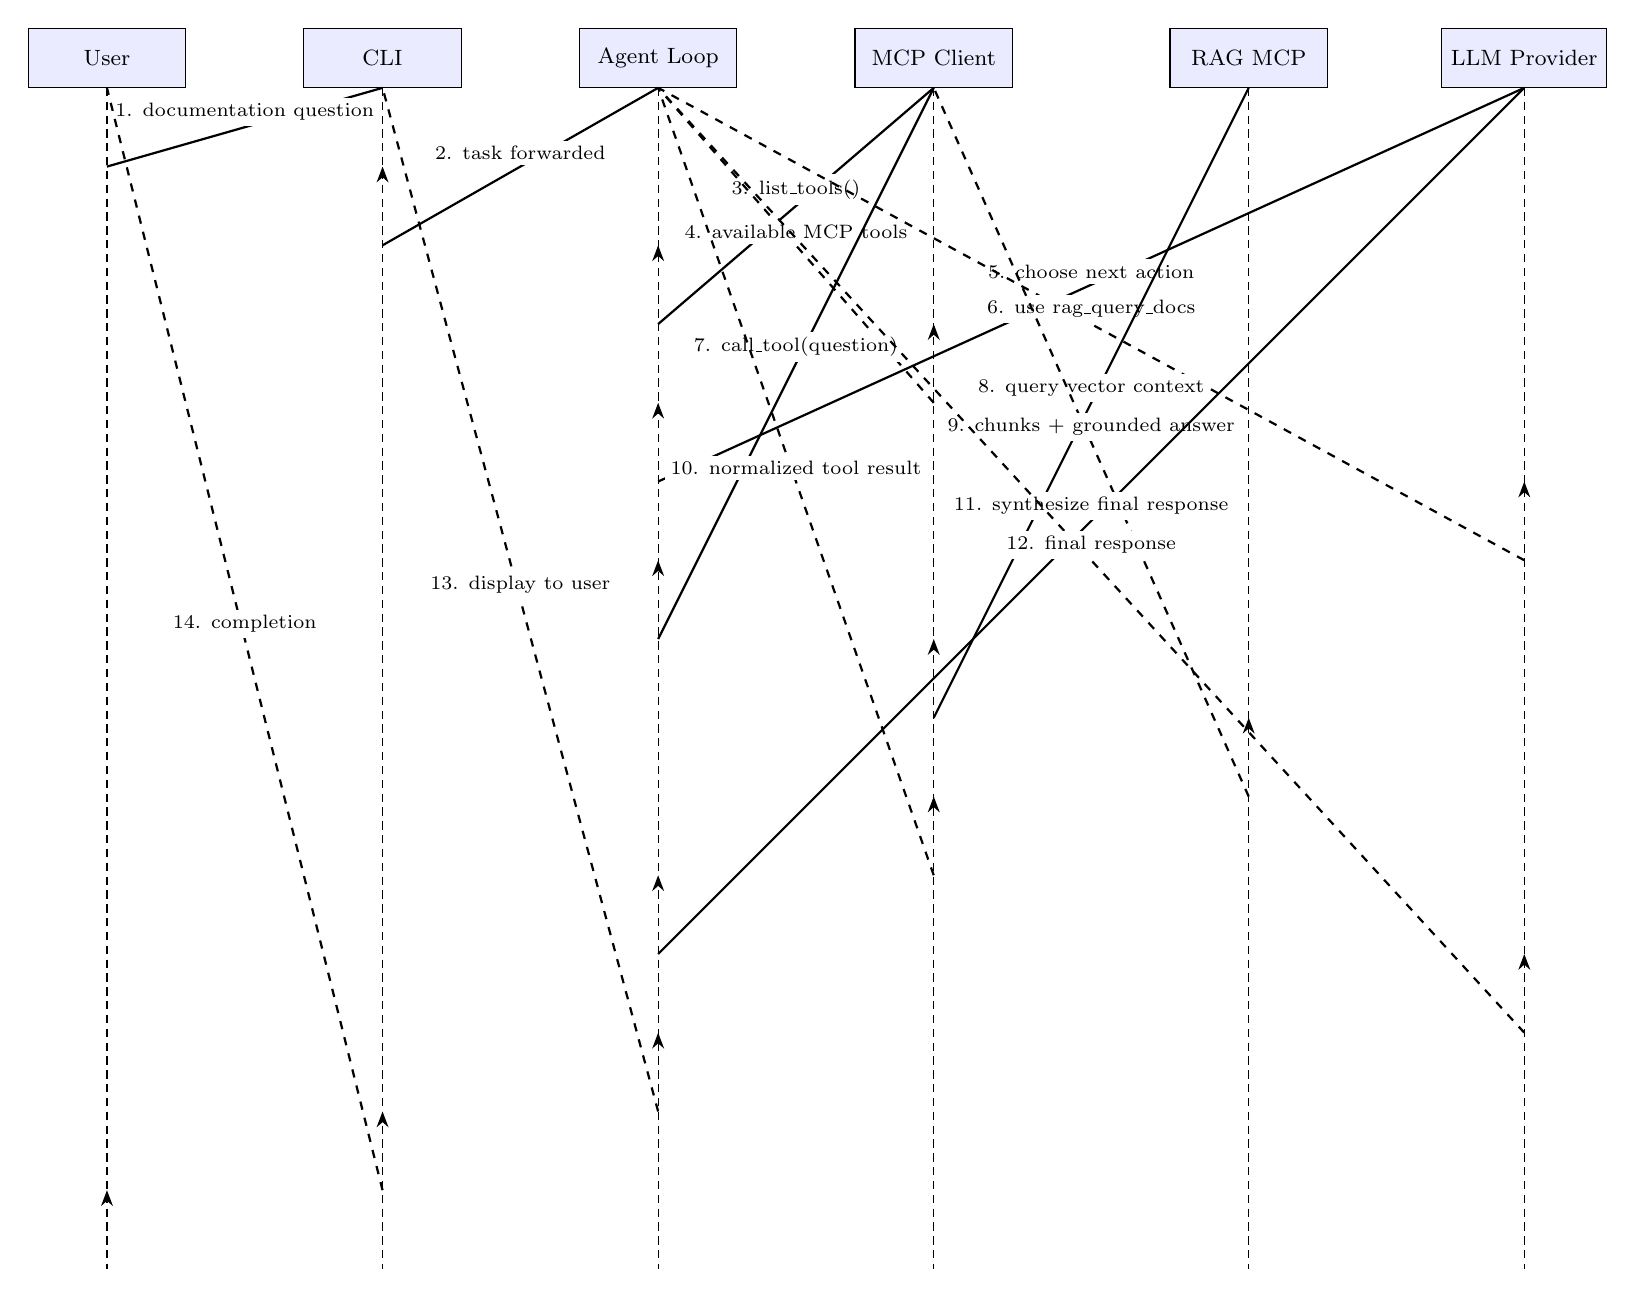
\begin{tikzpicture}[
  lifeline/.style={draw, minimum width=2.0cm, minimum height=0.75cm, align=center, font=\footnotesize, fill=blue!8},
  msg/.style={-{Stealth[length=2mm]}, thick},
  ret/.style={-{Stealth[length=2mm]}, thick, dashed},
  msglabel/.style={above, font=\scriptsize, fill=white, inner sep=2pt}
]
% Nodes (Horizontally spaced to accommodate longer text)
\node[lifeline] (u) at (0,0) {User};
\node[lifeline] (c) at (3.5,0) {CLI};
\node[lifeline] (a) at (7.0,0) {Agent Loop};
\node[lifeline] (m) at (10.5,0) {MCP Client};
\node[lifeline] (r) at (14.5,0) {RAG MCP};
\node[lifeline] (p) at (18.0,0) {LLM Provider};

% Lifeline dashed lines (Extended to cover all messages)
\foreach \x in {u,c,a,m,r,p}{\draw[densely dashed] (\x.south) -- ++(0,-15.0);} 

% Messages (Evenly spaced vertically and using the msglabel style)
\draw[msg] (u.south) ++(0,-1.0) -- node[msglabel]{1. documentation question} (c.south) ++(0,-1.0);
\draw[msg] (c.south) ++(0,-2.0) -- node[msglabel]{2. task forwarded} (a.south) ++(0,-2.0);
\draw[msg] (a.south) ++(0,-3.0) -- node[msglabel]{3. list\_tools()} (m.south) ++(0,-3.0);
\draw[ret] (m.south) ++(0,-4.0) -- node[msglabel]{4. available MCP tools} (a.south) ++(0,-4.0);
\draw[msg] (a.south) ++(0,-5.0) -- node[msglabel]{5. choose next action} (p.south) ++(0,-5.0);
\draw[ret] (p.south) ++(0,-6.0) -- node[msglabel]{6. use rag\_query\_docs} (a.south) ++(0,-6.0);
\draw[msg] (a.south) ++(0,-7.0) -- node[msglabel]{7. call\_tool(question)} (m.south) ++(0,-7.0);
\draw[msg] (m.south) ++(0,-8.0) -- node[msglabel]{8. query vector context} (r.south) ++(0,-8.0);
\draw[ret] (r.south) ++(0,-9.0) -- node[msglabel]{9. chunks + grounded answer} (m.south) ++(0,-9.0);
\draw[ret] (m.south) ++(0,-10.0) -- node[msglabel]{10. normalized tool result} (a.south) ++(0,-10.0);
\draw[msg] (a.south) ++(0,-11.0) -- node[msglabel]{11. synthesize final response} (p.south) ++(0,-11.0);
\draw[ret] (p.south) ++(0,-12.0) -- node[msglabel]{12. final response} (a.south) ++(0,-12.0);
\draw[ret] (a.south) ++(0,-13.0) -- node[msglabel]{13. display to user} (c.south) ++(0,-13.0);
\draw[ret] (c.south) ++(0,-14.0) -- node[msglabel]{14. completion} (u.south) ++(0,-14.0);
\end{tikzpicture}%
}
\caption{Sequence flow for documentation query grounded with local RAG.}
\end{figure}

\section{Sequence Diagram --- Scenario 2 (Read/Edit File Flow)}

\begin{figure}[H]
\centering
\resizebox{\textwidth}{!}{%
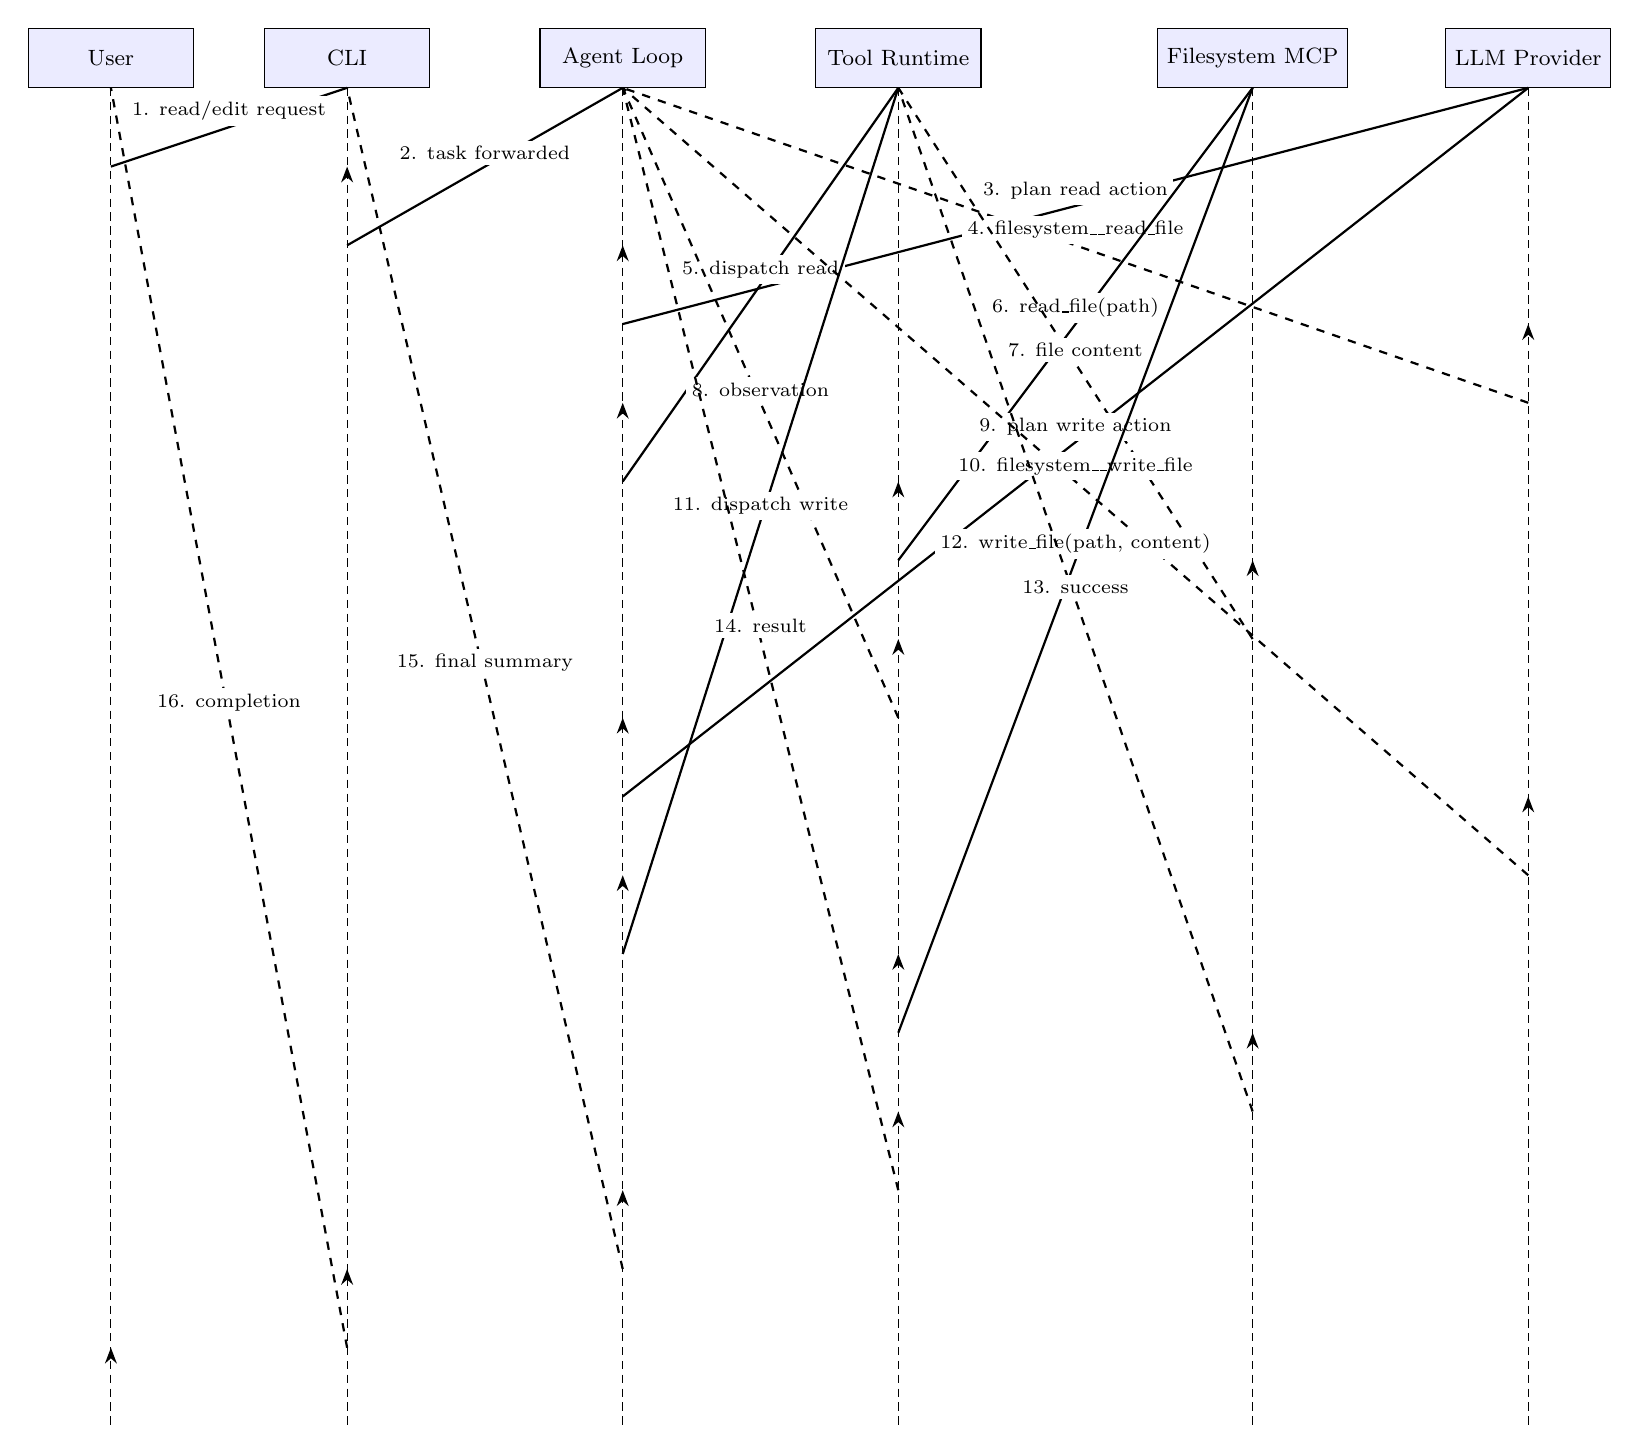
\begin{tikzpicture}[
  lifeline/.style={draw, minimum width=2.1cm, minimum height=0.75cm, align=center, font=\footnotesize, fill=blue!8},
  msg/.style={-{Stealth[length=2mm]}, thick},
  ret/.style={-{Stealth[length=2mm]}, thick, dashed},
  msglabel/.style={above, font=\scriptsize, fill=white, inner sep=2pt}
]
% Nodes (Horizontally spaced to accommodate longer text)
\node[lifeline] (u) at (0,0) {User};
\node[lifeline] (c) at (3.0,0) {CLI};
\node[lifeline] (a) at (6.5,0) {Agent Loop};
\node[lifeline] (t) at (10.0,0) {Tool Runtime};
\node[lifeline] (f) at (14.5,0) {Filesystem MCP};
\node[lifeline] (p) at (18.0,0) {LLM Provider};

% Lifeline dashed lines (Extended to cover all messages)
\foreach \x in {u,c,a,t,f,p}{\draw[densely dashed] (\x.south) -- ++(0,-17.0);} 

% Messages (Evenly spaced vertically and using the new msglabel style)
\draw[msg] (u.south) ++(0,-1.0) -- node[msglabel]{1. read/edit request} (c.south) ++(0,-1.0);
\draw[msg] (c.south) ++(0,-2.0) -- node[msglabel]{2. task forwarded} (a.south) ++(0,-2.0);
\draw[msg] (a.south) ++(0,-3.0) -- node[msglabel]{3. plan read action} (p.south) ++(0,-3.0);
\draw[ret] (p.south) ++(0,-4.0) -- node[msglabel]{4. filesystem\_\_read\_file} (a.south) ++(0,-4.0);
\draw[msg] (a.south) ++(0,-5.0) -- node[msglabel]{5. dispatch read} (t.south) ++(0,-5.0);
\draw[msg] (t.south) ++(0,-6.0) -- node[msglabel]{6. read\_file(path)} (f.south) ++(0,-6.0);
\draw[ret] (f.south) ++(0,-7.0) -- node[msglabel]{7. file content} (t.south) ++(0,-7.0);
\draw[ret] (t.south) ++(0,-8.0) -- node[msglabel]{8. observation} (a.south) ++(0,-8.0);
\draw[msg] (a.south) ++(0,-9.0) -- node[msglabel]{9. plan write action} (p.south) ++(0,-9.0);
\draw[ret] (p.south) ++(0,-10.0) -- node[msglabel]{10. filesystem\_\_write\_file} (a.south) ++(0,-10.0);
\draw[msg] (a.south) ++(0,-11.0) -- node[msglabel]{11. dispatch write} (t.south) ++(0,-11.0);
\draw[msg] (t.south) ++(0,-12.0) -- node[msglabel]{12. write\_file(path, content)} (f.south) ++(0,-12.0);
\draw[ret] (f.south) ++(0,-13.0) -- node[msglabel]{13. success} (t.south) ++(0,-13.0);
\draw[ret] (t.south) ++(0,-14.0) -- node[msglabel]{14. result} (a.south) ++(0,-14.0);
\draw[ret] (a.south) ++(0,-15.0) -- node[msglabel]{15. final summary} (c.south) ++(0,-15.0);
\draw[ret] (c.south) ++(0,-16.0) -- node[msglabel]{16. completion} (u.south) ++(0,-16.0);
\end{tikzpicture}%
}
\caption{Sequence flow for read/edit workflow through Tool Runtime and filesystem MCP.}
\end{figure}
\section{Execution Semantics}

\subsection{Agentic Loop}
The agent runs in bounded steps (\texttt{max\_steps}) and exchanges a strict structured format:
\texttt{thought}, \texttt{action}, and \texttt{final}. If an action is returned, the call is routed through
Tool Runtime; otherwise, completion or replanning occurs.

\subsection{Tool Runtime and Safety Modes}
\begin{itemize}
    \item \textbf{Confirm mode}: each tool call requires user approval before execution.
    \item \textbf{Auto mode}: tool calls execute directly for faster workflows.
\end{itemize}

Both local and MCP tool calls share one dispatch path, ensuring consistent logging and control.

\subsection{Provider Abstraction and Fallback}
Provider selection is based on environment settings. If a selected provider is unavailable,
fallback selection is attempted so the CLI remains operational. Runtime provider failures are
captured and surfaced as non-crashing error text.

\section{Validation and Testing}

\begin{itemize}
    \item End-to-end usage validated through CLI run mode and REPL mode.
    \item MCP integrations validated across filesystem, context7, and local rag server paths.
    \item Deployment documentation and checklist maintained in \texttt{DEPLOYMENT.md}.
    \item Usage and recovery paths documented in \texttt{HOW\_TO\_USE.md}.
\end{itemize}

\begin{table}[H]
\centering\small
\begin{tabularx}{\textwidth}{@{}l l X@{}}
\toprule
\textbf{Area} & \textbf{Status} & \textbf{Evidence} \\
\midrule
Automated tests & Pass & \texttt{pytest -q} run in project environment \\
Deployment flow & Documented & \texttt{DEPLOYMENT.md} with checks and post-deploy checklist \\
User workflow docs & Updated & \texttt{HOW\_TO\_USE.md} with working REPL/run commands \\
Demo artifact & Present & \texttt{docs/demo/demo-video.mp4} \\
\bottomrule
\end{tabularx}
\caption{Validation status summary.}
\end{table}

\section{Limitations and Future Work}

\begin{itemize}
    \item Provider/model quality depends on quota, capacity, and API behavior.
    \item Some hosted models may produce incompatible tool-calling outputs.
    \item Next step: add stricter markdown quality rubric + validation pass in agent loop.
    \item Next step: extend benchmark suite for retrieval quality metrics across larger corpora.
    \item Next step: add deterministic schema validation before finalizing generated documentation.
\end{itemize}

\section{Conclusion}

ForgePilot delivers a practical and extensible CLI assistant architecture by combining
agentic planning, safe runtime execution, MCP tool orchestration, and local RAG grounding.
The implemented design balances usability (run/repl workflows), safety (confirm mode), and
automation (auto mode) while preserving traceability through logs, docs, and structured tool calls.

The current implementation is deployment-ready for coursework/demo scenarios and provides a
clear baseline for future improvements in retrieval evaluation, prompt quality controls, and
provider interoperability.

\appendix
\section{Artifact Index}

\begin{itemize}
    \item Architecture narrative: \texttt{ARCHITECTURE.md}
    \item State diagram source: \texttt{docs/planning/STATE\_DIAGRAM.mmd}
    \item Sequence source 1: \texttt{docs/planning/SEQUENCE\_SCENARIO\_1\_DOC\_RAG.mmd}
    \item Sequence source 2: \texttt{docs/planning/SEQUENCE\_SCENARIO\_2\_READ\_EDIT.mmd}
    \item Deployment guide: \texttt{DEPLOYMENT.md}
    \item Usage guide: \texttt{HOW\_TO\_USE.md}
\end{itemize}

\end{document}
